\documentclass[conference]{IEEEtran}
\IEEEoverridecommandlockouts
% The preceding line is only needed to identify funding in the first footnote. If that is unneeded, please comment it out.
\usepackage{cite}
\usepackage{url}
\usepackage{amsmath,amssymb,amsfonts}
\usepackage{algorithmic}
\usepackage{graphicx}
\usepackage{textcomp}
\usepackage{xcolor}
\def\BibTeX{{\rm B\kern-.05em{\sc i\kern-.025em b}\kern-.08em
    T\kern-.1667em\lower.7ex\hbox{E}\kern-.125emX}}
\begin{document}

\title{Network Data Collection for Artifical Intelligence
}

\author{\IEEEauthorblockN{Sebastian Lipp}
\IEEEauthorblockA{\textit{IT Security} \\
\textit{FH Technikum Wien}\\
Vienna, Austria \\
cs19m032@technikum-wien.at}
\and
\IEEEauthorblockN{Damir Marijanovic}
\IEEEauthorblockA{\textit{IT Security} \\
\textit{FH Technikum Wien}\\
Vienna, Austria \\
cs19m031@technikum-wien.at}
\and
\IEEEauthorblockN{Boris Stampf}
\IEEEauthorblockA{\textit{IT Security} \\
\textit{FH Technikum Wien}\\
Vienna, Austria \\
cs19m006@technikum-wien.at}
}

\maketitle

\begin{abstract}
Collecting real network data for further processing is an important topic for the training of neuronal networks which filter suspicious from ordinary traffic. This paper focuses mainly on research in the areas of network simulation, network recording and data extraction which should serve as input for the following papers.
\end{abstract}

\begin{IEEEkeywords}
artifical intelligence, neuronal networks, computer networks, network security, data collection
\end{IEEEkeywords}

\section{Introduction}
Neuronal networks which filter suspicious network traffic need a training data set of high quality. This data set could be produced from real network traffic but this can be difficult to implement. Another option considers network simulators which can be easily configured depending on the selected scenarios.

This paper is split in three chapters. The first chapter compares available network simulators and their software interfaces and explores possibilities for their automated setup based on the scenario and parameters. The second chapter focuses on tools to record the network traffic. In the third chapter methods of feature extraction and label definition are covered. This information serves as foundation for the further implementation of a system for automated data collection for artifical intelligence.

At this point all our considerations are based on theoretical research  without practical implementation which will come to life in further work. Therefore this paper sets a direction and foundation for the next steps and shows possible solutions on a high level.

\section{Simulation}

Before network simulators can be compared the requirements have to be defined. Because the produced network traffic should be close to real traffic it would be advisable to choose a network simulator which works with the simulation of real network equipment and can also integrate real hardware or virtual machines into the simulation which is necessary to redirect the network traffic to the recorder and data extractor. This is important to consider since other simulators like NS3 provide discrete-event network simulation which is a needless complexity overhead for this kind of application. It would be desirable if they are affordable and provide an easy-to-use interface to create and control specific network topologies through a programming language like Python to automate their creation. Moreover they should be resource-efficient and easy to deploy. The provisioning of the simulation hosts has to be simple and also scalable to be prepared for simulating denial-of-service attacks.

The next sections cover possible network simulators, system environments and the provisioning of the infrastructure.

\subsection{Comparing common network simulators}
There are many solutions available on the market to simulate networks. Popular network simulators which possibly fulfill the requirements above are for example VIRL, GNS3 or EVE-NG. This section focuses on the comparison of these simulators and the selection of the best solution for our use case.  \cite{b1}

\begin{figure}[htbp]
\centerline{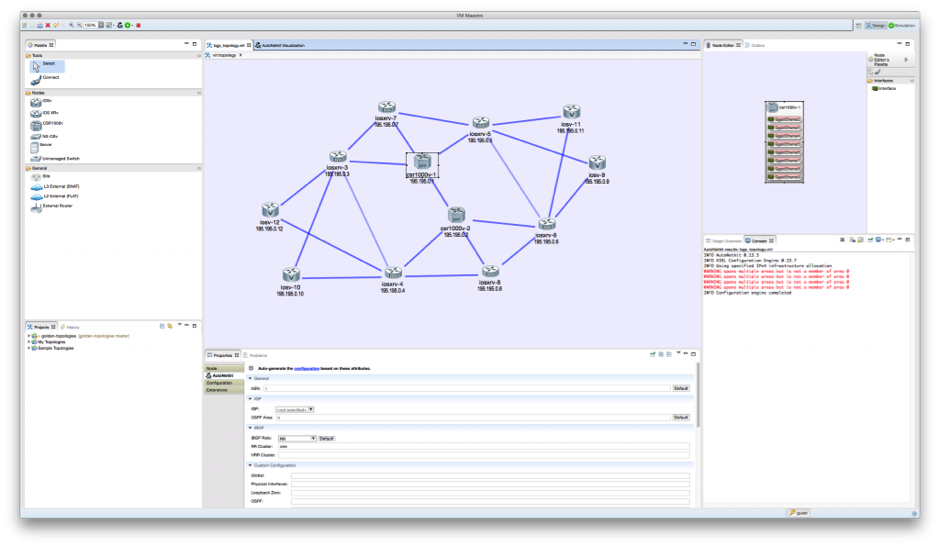
\includegraphics[scale=0.55]{virl.png}}
\caption{Sample network topology in VIRL \cite{b2}}
\label{virl}
\end{figure}

VIRL (Cisco Virtual Internet Routing Lab) is a network modeling and simulation environment provided by Cisco which offers the ability to use simulation models of real Cisco platforms, integrate virtual machines and connect real networks. Furthermore it provides a RESTful API to configure networks without a graphical interface, sufficient documentation and scalability as well as easy deployment through prepared images. It is not for free and only supports VMware or bare-metal installs. Simulation models of other vendors are not supported. Tests in virtual machines unveiled a good responsiveness but a long topology loading time with high CPU load. Fig.~\ref{virl} shows a sample network topology created via the graphical user interface of VIRL.  \cite{b1} \cite{b3}

\newpage

\begin{figure}[htbp]
\centerline{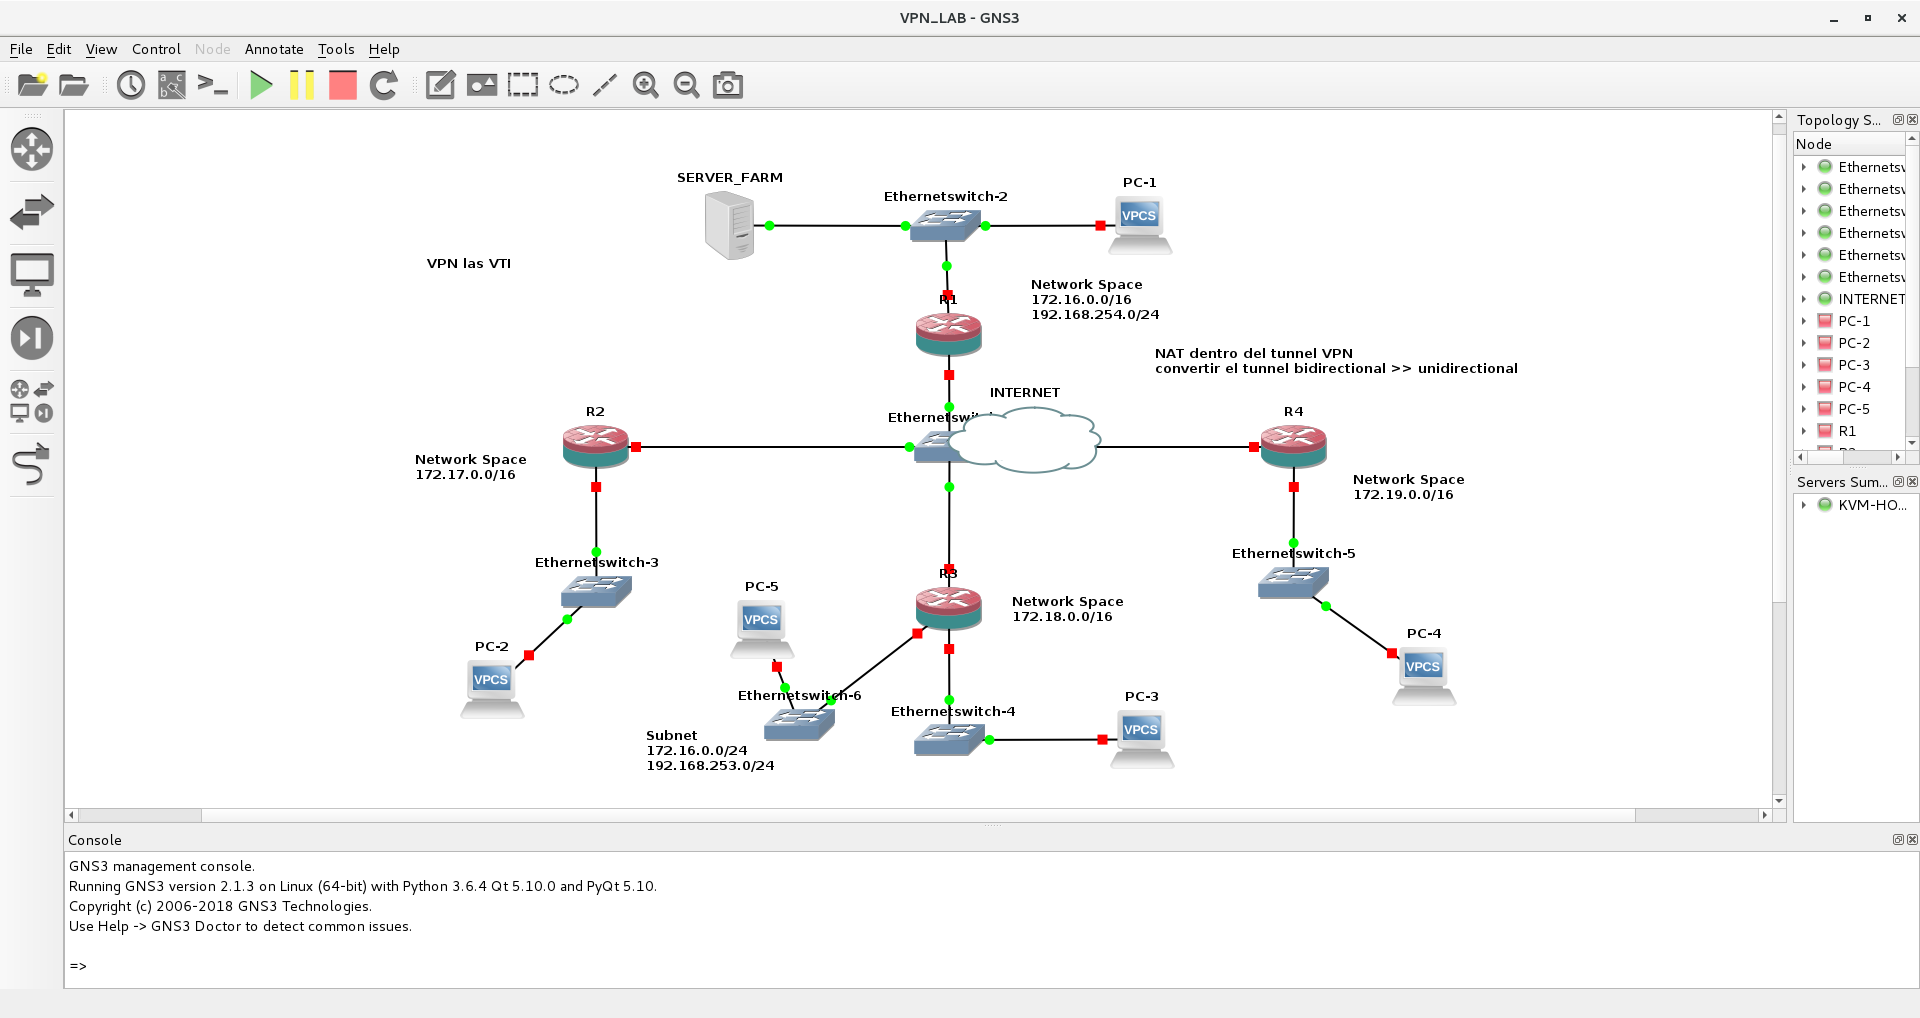
\includegraphics[scale=0.13]{gns3.png}}
\caption{Sample network topology in GNS3 \cite{b4}}
\label{gns3}
\end{figure}

GNS3 (Graphical Network Simulator 3) is a very popular free open source software to emulate and test networks. It offers the integration of virtual machines and real networks and supports models of various vendors but does not offer pre-installed device images due to license issues. It also provides a RESTful API to setup network topologies, a big community and scalability. The software can be easily installed through packages on all operating systems and supports all hypervisors as well Docker containers. Performance tests showed a long topology loading time with high CPU load but a good response through the user interface. Fig.~\ref{gns3} shows a sample network topology created with GNS3.  \cite{b1} \cite{b5}

\begin{figure}[htbp]
\centerline{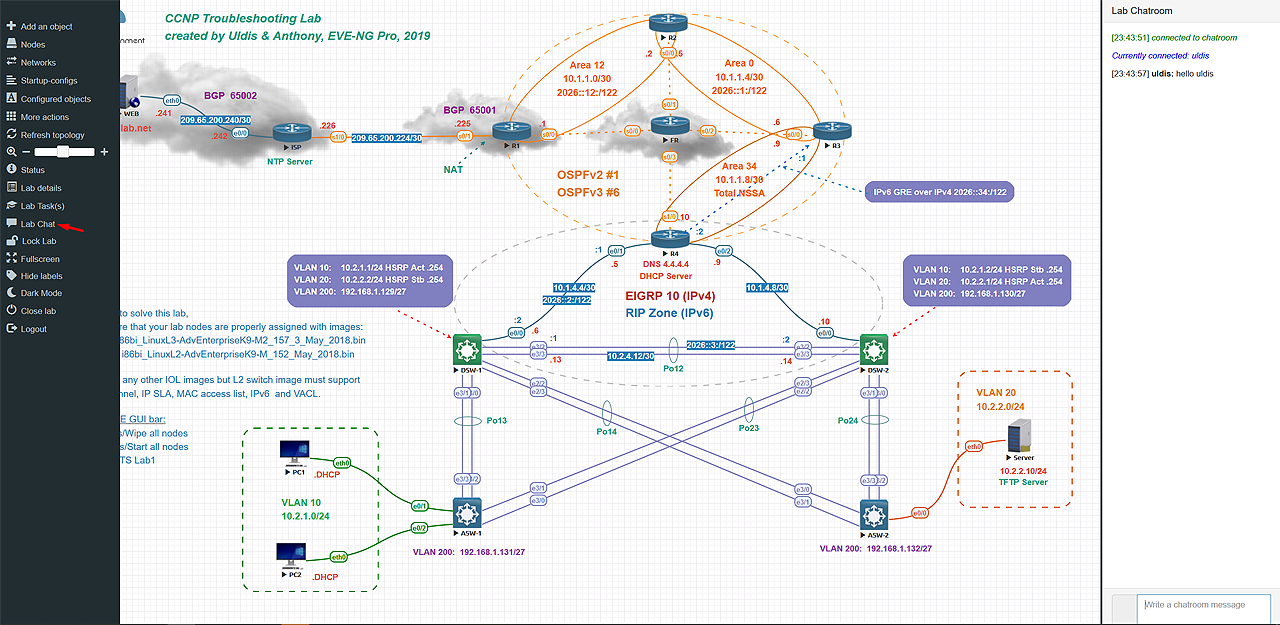
\includegraphics[scale=0.19]{eve-ng.png}}
\caption{Sample network topology in EVE-NG \cite{b6}}
\label{eve-ng}
\end{figure}

EVE-NG (Emulated Virtual Environment - Next Gen) is a network emulator which comes in a free and a professional edition and offers the interaction with real networks. It supports multiple vendors but does not provide device images. Advanced features like Docker, configuration management or Wireshark integration only come with the purchase version. Moreover a RESTful API and images for the installation in virtual machines are available as well as a reasonable documentation. The software is scalable and performs well in virtual machines with a short topology loading time and provides an intuitive interface as shown in Fig.~\ref{eve-ng}.  \cite{b1} \cite{b7}

All solutions are very similar in their functionalities but distinguish in their vendor support, performance, documentation and price. VIRL only supports Cisco devices but comes with device images like GNS3 and EVE-NG support various vendors but do not ship images. But many proprietary and open source images are available on the internet for free. VIRL and EVE-NG are propriatary like GNS3 is free and open source. EVE-NG performs better in virtual machines than VIRL and GNS3.

Regarding these factors GNS3 fullfills our requirements the most because it is free, supports all vendors and comes with a big community and documentation. Our second option would be EVE-NG in the professional edition which also supports all vendors.

\subsection{Selecting the deployment environment}

Next steps include the integration of the selected network simulator in a scalable environment which can be set up easily. 

\begin{figure}[htbp]
\centerline{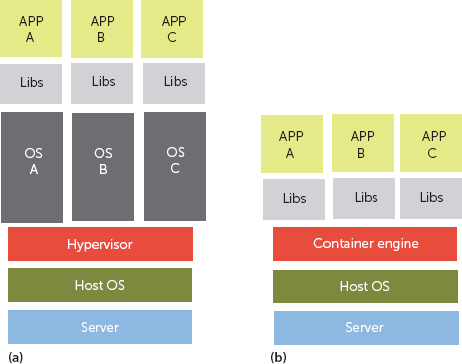
\includegraphics[scale=0.25]{docker_vm.png}}
\caption{Virtual machines vs. Containers \cite{b8}}
\label{docker-vm}
\end{figure}

Hypervisors like VirtualBox or VMware provide the possibility to setup full virtual computers on a physical host where Docker containers are encapsuled sandboxes on an existing operating system like illustrated in Fig.~\ref{docker-vm}. It is clear that containers are more resource efficent but in virtual machines the systems are better isolated. In our case we could use both solutions because the network simulators are also capable to run in Docker containers. If we focus on resource efficency and scalability also Kubernetes comes in our minds which is an orchestrator for deploying Docker containers on multiple nodes but it is a more complex configuration overhead and needs certain amount of hardware to unfold its potential also for simple scenarios. Because we want an affordable solutions which can be used in most of the cases also on our computers with some exceptions, we decided to use a tool which can create virtual machines as well as Docker containers to be ready for the future. Regarding the corner cases servers or a Kubernetes cluster could be rented temporarily on cloud platforms to support high-load scenarios e.g. big denial-of-service attacks.

A popular solution to bootstrap development environments in virtual machines is called Vagrant which provides lightweight base images and an interface to automate the configuration of the virtual machines. Moreover it can be connected to provisioning tools to further configure host systems. Vagrant supports VirtualBox or VMware but also Docker and can be extended to support cloud services like AWS or even to install a whole Kubernetes cluster. It gives us the power to start with simple configurations and scale them up to more sophisticated ones using containerization and complex orchestrators. \cite{b9}

This means we are ready to create system environments on our host or in the cloud and install base systems on them. The next section focuses on the automated setup of the network simulator, recorder and data extractor within virtual machines or Docker containers as well as the configuration of network topologies based on the selected scenarios and parameters to produce, record and extract network traffic for further processing in neuronal networks to improve their strike rate.

\subsection{Provisioning of the infrastructure}

Vagrant supports multiple provisioners like Ansible, Terraform or simple bash scripts to configure the host systems and can also be set up through them. For the beginning we will use Ansible through Vagrant to configure the host system. Vagrant can setup multiple virtual machines or Docker containers on one host. If we would need to set up machines on multiple hosts we will come back to tools like Terraform for example. \cite{b9}

If all the possible network scenarios are defined these network topologies have to be deployed through our deployment system consisting of Vagrant and Ansible. This means we will define the basic host setup and the network configurations for all the scenarios in Ansible templates which could be later adjusted via command line parameters. The topology can then be deployed by executing a shell command. This includes the deployment of the network recorder and the data extractor. In other words one or multiple scenarios can be started and connected to one recorder and data extractor to combine simultaneous attacks and everything will be deployed through a shell command with static configuration in templates and dynamic configuration with command line options. It will be also possible to integrate real hardware into the simulation.

\begin{figure}[htbp]
\centerline{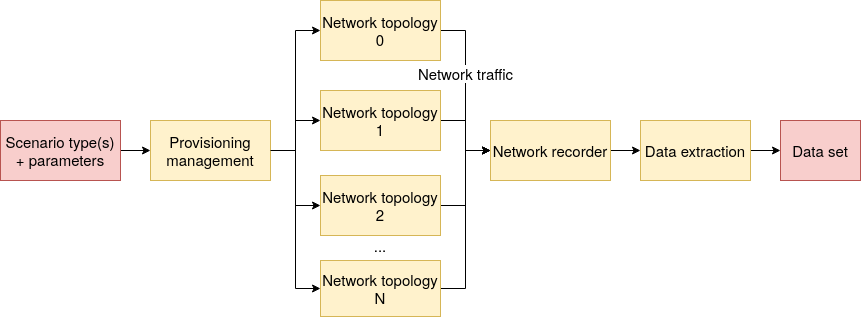
\includegraphics[scale=0.28]{design_flow.png}}
\caption{Data collection workflow}
\label{design-flow}
\end{figure}

Fig.~\ref{docker-vm} shows a schematic overview of the simulation workflow. The input parameters are the type of scenario(s) and the respective settings which deploys hosts including the base systems and the simulators applying the network topologies. Moreover the network recorder and data extractor will be deployed to gather the network traffic and extract the features to create data sets which could be collected in a central database.

A real test case would then consist of multiple scenarios of attacks and usual network traffic recorded, extracted and collected in a central place. The next chapter focuses on recording the generated data.

\section{Recording}

\section{Data Extraction}

\begin{thebibliography}{00}
\bibitem{b1} CBT Nuggets Blog (2020). 5 Best Network Simulators for Cisco Exams: CCNA, CCNP, CCIE. [online] Available at: \newline\url{https://www.cbtnuggets.com/blog/career/career-progression/5-best-network-simulators-for-cisco-exams-ccna-ccnp-and-ccie} [Accessed 22 Feb. 2020].
\bibitem{b2} Network Computing. (2020). Cisco VIRL: More Than A Certification Study Lab. [online] Available at: \url{https://www.networkcomputing.com/networking/cisco-virl-more-certification-study-lab} [Accessed 22 Feb. 2020].
\bibitem{b3} Virl.cisco.com. (2020). VIRL Getting Started Tutorial. [online] Available at: \url{http://virl.cisco.com/virl.apis.php} [Accessed 22 Feb. 2020].
\bibitem{b4} Gns3.com. (2020). GNS3 | The software that empowers network professionals. [online] Available at: \url{https://gns3.com/discussions/how-to-install-gns3-on-centos-7-} [Accessed 22 Feb. 2020].
\bibitem{b5} Gns3-server.readthedocs.io. (2020). Welcome to API documentation! — GNS3 2.1.22dev1-67e70c46 documentation. [online] Available at: \url{https://gns3-server.readthedocs.io/en/latest/} [Accessed 22 Feb. 2020].
\bibitem{b6} Eve-ng.net. (2020). Screenshots. [online] Available at: https://www.eve-ng.net/index.php/screenshots/ [Accessed 22 Feb. 2020].
\bibitem{b7} Eve-ng.net. (2020). EVE-NG API. [online] Available at: \url{https://www.eve-ng.net/index.php/documentation/howtos/how-to-eve-ng-api/} [Accessed 22 Feb. 2020].
\bibitem{b8} SOSC-2018. (2020). Docker. [online] Available at: \url{https://dodas-ts.github.io/SOSC-2018/docker.html} [Accessed 22 Feb. 2020].
\bibitem{b9} Chan, M. (2020). 15 Infrastructure as Code Tools to Automate Deployments - Thorn Tech. [online] Thorn Technologies. Available at: \url{https://www.thorntech.com/2018/04/15-infrastructure-as-code-tools/} [Accessed 22 Feb. 2020].
\end{thebibliography}
\vspace{12pt}
\color{red}
\end{document}


